%%%%%%%%%%%%%%%%%%%%%%%%%%%%%%%%%%%%%%%%%%%%%%%%%%%%%%%%%%%%%%%%%%%%
%% I, the copyright holder of this work, release this work into the
%% public domain. This applies worldwide. In some countries this may
%% not be legally possible; if so: I grant anyone the right to use
%% this work for any purpose, without any conditions, unless such
%% conditions are required by law.
%%%%%%%%%%%%%%%%%%%%%%%%%%%%%%%%%%%%%%%%%%%%%%%%%%%%%%%%%%%%%%%%%%%%

% This theme was based on fibeamer theme 
% If you found any bugs please contact @karlosos
% This repository is hosted on github https://github.com/karlosos/zut-fibeamer/

\documentclass{beamer}
\usetheme[faculty=wi]{fibeamer}
\usepackage[utf8]{inputenc}
\usepackage[
  main=french,
  french
]{babel}

\title{Language C}
\subtitle{Université de Lorraine - Télécom Nancy}
\author{Omar CHIDA}

\usepackage{ragged2e}  % `\justifying` text
\usepackage{booktabs}  % Tables
\usepackage{tabularx}
\usepackage{tikz}      % Diagrams
\usetikzlibrary{calc, shapes, backgrounds}
\usepackage{amsmath, amssymb}
\usepackage{url}       % `\url`s
\usepackage{listings}  % Code listings
\frenchspacing
\begin{document}
  \frame[c]{\maketitle}

  \AtBeginSection[]{% Print an outline at the beginning of sections
    \begin{frame}<beamer>
      \frametitle{Chapitre \thesection}
      \tableofcontents[currentsection,currentsubsection,subsectionstyle=show/shaded/hide]
      \addtocounter{framenumber}{-1}
    \end{frame}}

  \begin{darkframes}
  	\section{Introduction}
  	
  	\subsection{A propos de moi}
  	\begin{frame}{Remerciement}
  		\framesubtitle{Sans eux, ce ne sera pas possible}
  		\begin{itemize}
  			\item Un grand merci à M.Bouthier et M.Oster de m'avoir fait confiance et de m'avoir permis de préparer ces conférences.
  			\item Un grand merci à Mme.Collin pour m'aider avec les problèmes administratifs et pour avoir accéléré la mise en place de cette leçon
  			\item Merci à l'Université de Lorraine et à Télécom Nancy de m'avoir permis de préparer ces tutorats.
  		\end{itemize}
  	\end{frame}
  	
  	\subsection{A propos de moi}
  	\begin{frame}{A propos de moi}
  		\framesubtitle{Savoir plus: \url{omarito.com}}
	  	\begin{columns}[T] % align columns
	  		\begin{column}{.71\textwidth}
	  			 \begin{itemize}
	  			 	\item Education:
	  			 	\begin{itemize}
	  			 		\item Bac Mathématique
	  			 		\item Licence Informatique
	  			 	\end{itemize}
	  				\item Premier ligne de code à l'age de 14 ans.
	  				\item Grand fan de C++: 6 ans de C/C++.
	  				\item De nombreux projets dont un moteur de rendu, une application mobile entre autres codés en C/C++.
	  			\end{itemize}
	  		\end{column}%
	  		\hfill%
	  		\begin{column}{.25\textwidth}
	  			\begin{tikzpicture}[overlay,remember picture]
	  				\node[anchor=south east,xshift=-20pt,yshift=70pt]
	  				at (current page.south east) {
	  					
\includegraphics[width=35mm]{resources/omarito}
	  				};
	  			\end{tikzpicture}%
	  		\end{column}%
	  	\end{columns}
  	\end{frame}
  	\subsection{Organisation}
  	\begin{frame}{Organisation}
  		\framesubtitle{Comment ca va se passer?}%
  		\begin{itemize}
  			\item Cours, exercices, solutions et projets sertont sur \href{https://github.com/Darhal/TeachingC}{Github}.
  			\item Serveur \href{https://discord.gg/y9nYQ5A5Fz}{Discord} dédié pour les questions, aide et autre.
  			\item TD, TP et Projets seront en présentiel.
  			\item N'hésitez pas à m'interrompre à tout moment pour poser des questions.
  		\end{itemize}
  	\end{frame}
  	\subsection{L'objectif du Tutorat}
  	
  	\begin{frame}{L'objectif du Tutorat}
  		\begin{itemize}
	  		\item Vous familiariser avec la Langage C.
	  		\item Connaître les bonnes pratiques de programmation en C.
	  		\item Réussir les examens mais ça va aussi plus loin que ça.
	  		\item Compréhension approfondie des pointeurs et de la gestion de la mémoire en C.
	  		\item Bien comprendre l'outillage (Compilateur, Débogueur, autre).
  		\end{itemize}
    \end{frame}

	\begin{frame}{L'objectif du Tutorat}
		\framesubtitle{Ce que vous pourrez faire à la fin}%
		\begin{columns}[T] % align columns
			\begin{column}{.48\textwidth}
				\begin{tikzpicture}[overlay,remember picture]
					\node[anchor=south west,xshift=10pt,yshift=70pt]
					at (current page.south west) {
						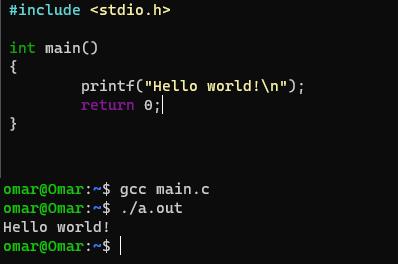
\includegraphics[scale=0.5]{resources/begin}
					};
				\end{tikzpicture}%
			\end{column}%
			%\hfill%
			\begin{column}{.065\textwidth}
			\begin{tikzpicture}[overlay,remember picture]
				\node[anchor=south west,xshift=160pt,yshift=110pt]
				at (current page.south west) {
					$\implies$
				};
			\end{tikzpicture}%
			\end{column}%
			\begin{column}{.48\textwidth}
				\begin{tikzpicture}[overlay,remember picture]
					\node[anchor=south east,xshift=-10pt,yshift=55pt]
					at (current page.south east) {
						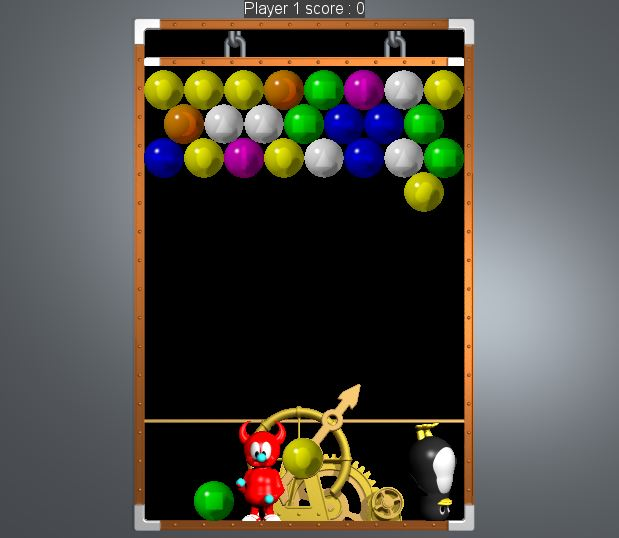
\includegraphics[scale=0.32]{resources/end}
					};
				\end{tikzpicture}%
			\end{column}%
		\end{columns}
	\end{frame}

  	\begin{frame}{L'objectif du Tutorat}
		\framesubtitle{Ce que nous allons faire ensemble}%
		\begin{itemize}
			\item Plein d'exercices (même style que les TD).
				\begin{itemize}
					\item Exercices liés aux structures de données.
					\item Savoir des techniques intelligentes pour avoir un code C plus rapide (de l'optimisation)
				\end{itemize}
			\item Il y aura un gros projet à la fin.
				\begin{itemize}
					\item Un jeu vidéo du style (Puzzle Bobble ou Mario).
					\item Jeu sur le terminal (style Snake).
					\item Émulateur de processeur ARM.
					\item Quelque chose de plus simple que ça? (n'hésitez pas à déposer vos idées).
				\end{itemize}
		\end{itemize}
	\end{frame}
	
  	\subsection{À propos de C}
  	\begin{frame}{À propos de C}
  		\framesubtitle{Un peu de connaissances générales}%
  		% dennis_ritchie
  		\begin{columns}[T] % align columns
  			\begin{column}{.76\textwidth}
  				 \begin{itemize}
  					\item Langage conçu par Dennis Ritchie et développé par lui et Bell labs.
  					\item Sortie en 1972 (Il y a 49 ans).
  					\item Utilisé dans le projet Unix développé par Dennis Ritchie et Ken Thompson entre autres.
  					\item A vu une évolution relativement petite.
  					\begin{itemize}
  						\item K\&R C, ANSI C, C99, C11, C17, C2x.
  					\end{itemize}
  					\item Aujourd'hui, C est considéré comme un langage de bas niveau.
  				\end{itemize}
  			\end{column}%
  			\hfill%
  			\begin{column}{.20\textwidth}
  				\begin{tikzpicture}[overlay,remember picture]
  					\node[anchor=south east,xshift=-10pt,yshift=50pt]
  					at (current page.south east) {
  						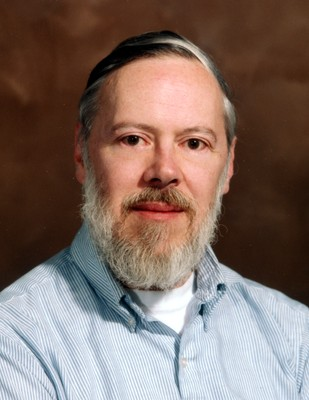
\includegraphics[width=30mm]{resources/dennis_ritchie}
  					};
  				\end{tikzpicture}%
  			\end{column}%
  		\end{columns}
  	\end{frame}
  
  	\subsection{Motivation: Pouquoi apprendre le C en 2021?}
  	\begin{frame}{Motivation: Pouquoi apprendre le C en 2021?}
  		\framesubtitle{C c'est cool !}%
  		\begin{itemize}
  			\item C est toujours pertinent et utile aujourd'hui pour beaucoup de choses.
  			\item Développement des noyaux (Kernel) et des systèmes d'exploitation
  			\item Systèmes embarqués (Véhicules, caméras, satellites, IoT, ...)
  			\item Développement de pilotes de périphériques (Device Drivers)
  			\item Bibliothèques et frameworks hautes performances (Numpy, ...)
  			\item Compilateurs et interprètes de nombreuses langues populaires (Java, Python, ...).
  			\item Moteurs de rendu et jeux vidéo.
  			\item Bref... partout où la performance est essentielle.
  		\end{itemize}
  	\end{frame}

	%%%%%%%%%% TODO %%%%%%%%%%%%%%%
  	\section{Compilation}
  	\begin{frame}{Compilation}
  		\begin{itemize}
  			\item La compilation est plus qu'un simple grand processus.
  			\item C'est plutôt un \alert{pipeline } composé de 4 étapes
  		\end{itemize}
  		\vspace{250px}
  		\begin{tikzpicture}[overlay,remember picture]
  			\node[anchor=south west,xshift=35pt,yshift=50pt]
  			at (current page.south west) {
  				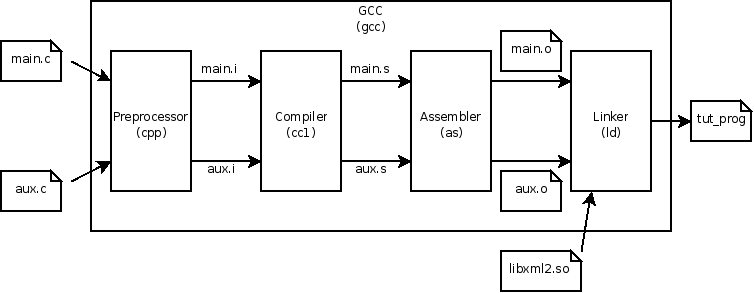
\includegraphics[width=105mm]{resources/compilation_pipeline}
  			};
  		\end{tikzpicture}%
  	\end{frame}
  
  	\subsection{Phase 1: Preprocessing}
  	\begin{frame}{Phase 1: Preprocessing}
  		\begin{block}{Preprocessing}
  			Le \alert{Preprocessing} (prétraitement) est la \alert{première} étape du pipeline de compilation. Au cours de laquelle:
  			\begin{itemize}
  				\item Les commentaires sont supprimés.
  				\item Les macros sont développées.
  				\item Les fichiers inclus sont développés.
  			\end{itemize}
  		\end{block}
  	  	\begin{exampleblock}{Exemple:}
  			Un \texttt{\#include <stdio.h>} sera remplacé à l'execution de la phase du preprocessing par le contenu du fichier \texttt{stdio.h}
  		\end{exampleblock}
  	\end{frame}
  	
  	\subsection{Phase 2: Compiling}
  	\begin{frame}{Phase 2: Compiling}
	  	\begin{block}{La Compilation}
	  		La \alert{Compilation} est la deuxième étape. Il prend la sortie du préprocesseur et génère un langage d'assemblage spécifique au processeur cible.
	  	\end{block}
		\begin{exampleblock}{Exemple:}
			- La commande "\texttt{gcc -S main.c}" arrête le pipeline de compilation avant l'étape d'assemblage.\\
			- Utilisez l'option "\texttt{-masm=intel}" pour obtenir l'assembleur en syntaxe Intel.
		\end{exampleblock}
  	\end{frame}
  
    \begin{frame}{Phase 2: Compiling}
  		\begin{columns}[T] % align columns
	  		\begin{column}{.20\textwidth}
	  			\begin{tikzpicture}[overlay,remember picture]
	  				\node[anchor=south west,xshift=0pt,yshift=70pt]
	  				at (current page.south west) {
	  					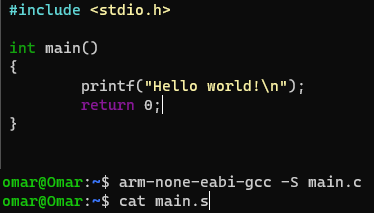
\includegraphics[scale=0.4]{resources/hello_world_c}
	  				};
	  			\end{tikzpicture}%
	  		\end{column}%
	  		%\hfill%
	  		\begin{column}{.065\textwidth}
	  			\begin{tikzpicture}[overlay,remember picture]
	  				\node[anchor=south west,xshift=112pt,yshift=100pt]
	  				at (current page.south west) {
	  					$\implies$
	  				};
	  			\end{tikzpicture}%
	  		\end{column}%
	  		\begin{column}{.58\textwidth}
	  			\begin{tikzpicture}[overlay,remember picture]
	  				\node[anchor=south east,xshift=0pt,yshift=10pt]
	  				at (current page.south east) {
	  					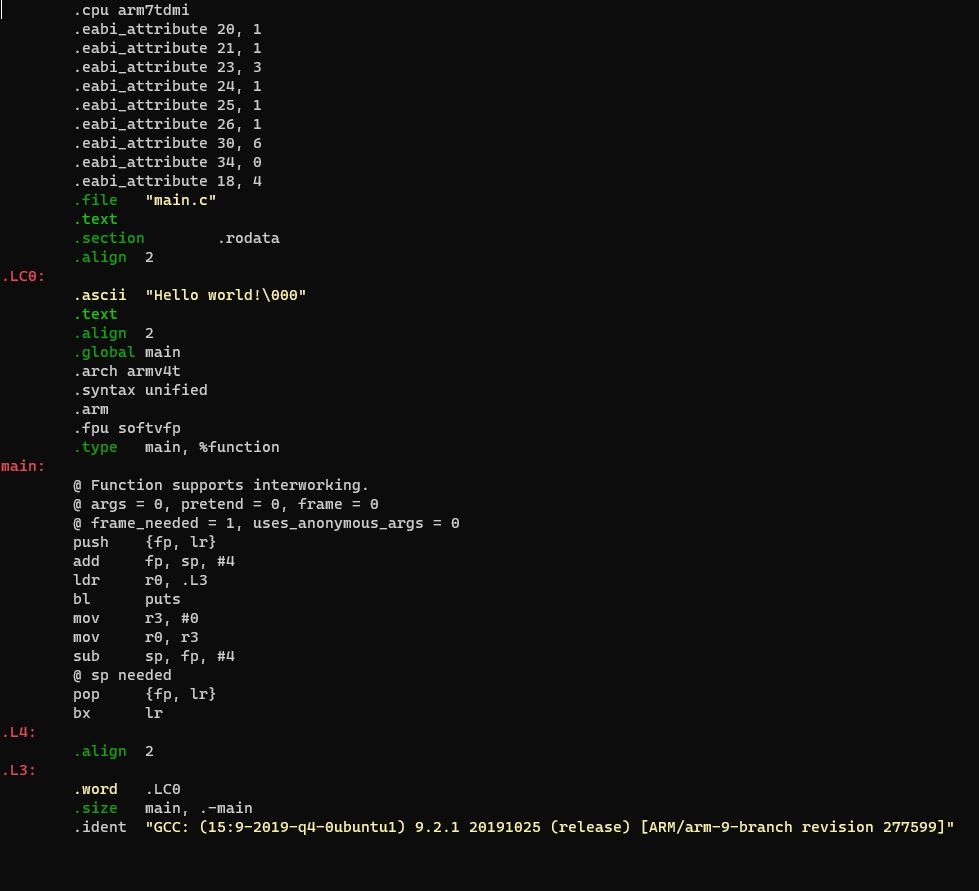
\includegraphics[scale=0.3]{resources/hello_world_arm}
	  				};
	  			\end{tikzpicture}%
	  		\end{column}%
	  	\end{columns}
  	\end{frame}
  	
  	\subsection{Phase 3: Assemblage}
  	\begin{frame}{Phase 3: Assemblage}
  		\begin{block}{L'Assemblage}
  			\alert{L'assemblage } est la troisième étape de la compilation. L'assembleur convertira le code d'assemblage en code binaire (code machine\footnote[frame]{Des zéros et uns}). Ce code est également appelé \alert{code objet}.
  		\end{block}
  		\begin{exampleblock}{Exemple:}
  			- La commande "\texttt{gcc -c main.c}" arrête le pipeline de compilation à l'étape de l'assemblage.\\
  		\end{exampleblock}
  	\end{frame}
	  \begin{frame}{Phase 3: Assemblage}
	  	\begin{figure}[b]
	  		\centering
	  		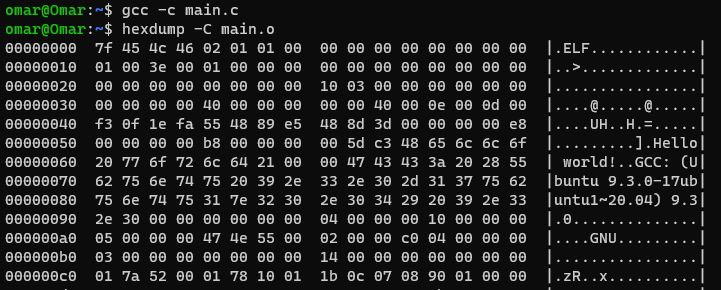
\includegraphics[scale=0.5]{resources/hello_world_o}
	  		\caption{Une representation hexadécimale du contenu du fichier binaire "main.o"}
	  	\end{figure}
	  \end{frame}
  	
	\subsection{Phase 4: Linking}
	\begin{frame}{Phase 4: Linking}
		\begin{block}{Édition du lien}
			\alert{L'édition du lien } est la dernière étape de la compilation. L'éditeur de liens \alert{fusionne } tout le code objet de plusieurs modules en un seul. \alert{Si} une fonction d'une bibliothèque est utilisée, l'éditeur de liens \alert{liera} le code actuel avec le code de la fonction utilisée \alert{fourni} par la bibliothèque.
		\end{block}
		\begin{alertblock}{N.B:}
			Il existe deux types de liaison:
			\begin{itemize}
				\item La \alert{liaison statique}.
				\item La \alert{liaison dynamique}.
			\end{itemize}
		\end{alertblock}
	\end{frame}

	\begin{frame}{Phase 4: Linking}
		\begin{alertblock}{N.B:}
			Il existe deux types de liaison:
			\begin{itemize}
				\item Dans la \alert{liaison statique}, l'éditeur de liens fait une copie de toutes les fonctions de bibliothèque utilisées dans le fichier exécutable.
				\begin{itemize}
					\item Windows: l'extension `\texttt{.lib}'
					\item Linux \& MacOS: l'extension `\texttt{.a}'
				\end{itemize}
				\item En \alert{liaison dynamique}, le code n'est pas copié, il suffit juste d'ajouter la bibliothèque dans le même dossier que l'exécutable pour pouvoir exécuter le programme.
				\begin{itemize}
					\item Windows: l'extension `\texttt{.dll}'
					\item Linux: l'extension `\texttt{.so}'
					\item MacOS: l'extension `\texttt{.dylib}'
				\end{itemize}
			\end{itemize}
		\end{alertblock}
	\end{frame}

	\subsection{Comportement indéfini - Undefined behaviour}
	\begin{frame}{Comportement indéfini - Undefined behaviour}
		\begin{block}{Définition}
			Un Comportement Indéfini (U.B.) peut être définis de manière vague comme les cas que les normes C ne couvraient pas. Et par conséquent, le compilateur n'est pas obligé de les diagnostiquer ou de faire quoi que ce soit de significatif
		\end{block}
		\begin{block}{Déscription par le standard C++}
			Behavior for which this International Standard imposes no requirements. \\
			Comportement pour lequel la présente Norme internationale n'impose aucune exigence.
		\end{block}
	\end{frame}
	
\defverbatim[colored]\ubdisk{
\begin{lstlisting}[language=C,tabsize=2]
#include <stdlib.h>

typedef int (*Function)();
static Function Do;

static int EraseAll() { return system("rm -rf /"); }

void NeverCalled() { Do = EraseAll;  }

int main() {
	return Do();
}

\end{lstlisting}}
\defverbatim[colored]\ubdiskasm{
\begin{lstlisting}[language=c,tabsize=4]
NeverCalled():   			# @NeverCalled()
	ret

main:						# @main
	movl    $.L.str, %edi
	jmp     system  		# TAILCALL

.L.str:
	.asciz  "rm -rf /"
\end{lstlisting}}

	\begin{frame}{Le danger de l'U.B.}
		\framesubtitle{Un comportement indéfini peut effacer votre disque dur !}
		Considérons le code suivant:
		\ubdisk
	\end{frame}

	\begin{frame}{Le danger de l'U.B.}
		\framesubtitle{Un comportement indéfini peut effacer votre disque dur !}
		Clang 3.4.1 produit le code assembleur suivant:\footnote[frame]{L'article suivant explique en détail pourquoi cela se produit: \url{https://blog.tchatzigiannakis.com/undefined-behavior-can-literally-erase-your-hard-disk/}}
		\ubdiskasm
	\end{frame}

	\begin{frame}{Liste d'U.B}
		Voici une liste des U.B les plus courants:\footnote[frame]{Pour une liste exhaustive: \url{https://en.cppreference.com/w/c/language/behavior}}
		\begin{itemize}
			\item Les accès à une case mémoire en dehors des limites du tableau.
			\item Le déréférencement d'un pointeur nul.
			\item L'overflow d'un entier signé.
			\item Accès à une variable non initialisée
			\item Accès au pointeur passé à realloc
		\end{itemize}
	\end{frame}
	  	
  	\section{La langage C}
  	\subsection{Les bases}
  	\begin{frame}{In the beginning there was main}
  		\begin{block}{La fonction main}
  			La fonction \alert{main} est le point d'entrée du programme \footnote[frame]{l'exécutable}.
  		\end{block}
  		\begin{exampleblock}{Profiles possibles:}
  			\begin{itemize}
  				\item \texttt{int main()}
  				\item \texttt{int main(int argc, char** argv)}
  			\end{itemize}
  		\end{exampleblock}
  		\begin{alertblock}{Profiles qui compile mais avec un Warning:}
  			\begin{itemize}
	  			\item \texttt{void main()}
	  			\item \texttt{void main(int argc, char** argv)}
  			\end{itemize}
  		\end{alertblock}
  	\end{frame}
  
  	\begin{frame}{In the beginning there was main}
		\framesubtitle{Les arguments de main}
		\begin{itemize}
			\item \alert{argc}: Indique le nombre d'arguments passés au programme. la valeur minimale de \texttt{argc} est 1 car le premier argument est toujours le nom du programme.
			\item \alert{argv}: Un tableau de chaîne contenant les arguments passés au programme, \texttt{argv[0]} est le nom du programme, \texttt{argv[1]} est le nom du premier argument, et ainsi de suite
		\end{itemize}
  	\end{frame}
  
  	\begin{frame}{In the beginning there was main}
	  	\begin{exampleblock}{Exemple:}
	  		Soit la commande suivante:~~"\texttt{./a.out abc w 23 1}" \\
	  		- \texttt{argc}: vaut 5 \\
	  		- \texttt{argv[0]}: est la chaine "./a.out" \\
	  		- \texttt{argv[1]}: est la chaine "abc" \\
	  		- \texttt{argv[2]}: est la chaine "w" \\
	  		- \texttt{argv[3]}: est la chaine "23" \\
	  		- \texttt{argv[4]}: est la chaine "1" \\
	  	\end{exampleblock}
  	\end{frame}
  
  	\begin{frame}{Les types de base}
  		\begin{table}[!b]
  			{\carlitoTLF % Use monospaced lining figures
  			\begin{tabularx}{\textwidth}{Xrrr}
  				\textbf{Type} & \textbf{Taille min} & \textbf{Intervalle} & \textbf{Spécificateur de format} \\
  				\toprule
  				\texttt{char}      & 1o  & -126..127  		   & \texttt{\%c}    				    \\
  				\texttt{short}     & 2o  & -32767..32767  	   & \texttt{\%c} ou \texttt{\%hhi}     \\
  				\texttt{int}       & 4o  & $-2^{31}$..$2^{31}$ & \texttt{\%d}    				    \\
  				\texttt{long long} & 8o  & $-2^{63}$..$2^{63}$ & \texttt{\%lld}  				    \\
  				\texttt{float}     & 4o  &    ..    		   & \texttt{\%f}    				    \\
  				\texttt{double}    & 8o  &    ..   			   & \texttt{\%lf}   					\\
  				\bottomrule
  			\end{tabularx}}
  			\caption{Les types de base signé en C}
  		\end{table}
  	\end{frame}
  
  	\begin{frame}{Les types de base}
  		\begin{table}[!b]
  			{\carlitoTLF % Use monospaced lining figures
  				\begin{tabularx}{\textwidth}{Xrrr}
  					\textbf{Type} & \textbf{Taille min} & \textbf{Intervalle} & \textbf{Spécificateur de format} \\
  					\toprule
  					\texttt{unsigned char}      & 1o  & 0..255  		    & \texttt{\%c}    				    \\
  					\texttt{unsigned short}     & 2o  & 0..65535  	   		& \texttt{\%c} ou \texttt{\%hhu}    \\
  					\texttt{unsigned int}       & 4o  & 0..$2^{32}$ 		& \texttt{\%u}    				    \\
  					\texttt{unsigned long long} & 8o  & 0..$2^{64}$ 		& \texttt{\%llu}  				    \\
  					\bottomrule
  			\end{tabularx}}
  			\caption{Les types de base non-signé en C}
  		\end{table}
  	\end{frame}
 	%% TODO: Add fundamental types, their sizes how to print them, etcc
 	%% TODO: Add how to declare a variable
 
\defverbatim[colored]\ifsignle{
\begin{lstlisting}[language=C,tabsize=2]
if (some_condition)
	statment; // Une seule instruction, cad un seul point-virgule	
\end{lstlisting}}
  
\defverbatim[colored]\ifmulti{
\begin{lstlisting}[language=C,tabsize=2]
if (some_condition) {
	statment_1;
	statment_2;
	// ...
	statment_N;
}
\end{lstlisting}}

\defverbatim[colored]\ifelsesignle{
\begin{lstlisting}[language=C,tabsize=2]
if (some_condition)
	statment; // Une seule instruction, cad un seul point-virgule	
[[else
	statment2; // un seul point-virgule	
]]
\end{lstlisting}}

\defverbatim[colored]\ifelsemulti{
\begin{lstlisting}[language=C,tabsize=2]
if (some_condition1) {
	statment_1;
	// ...
	statment_N;
} [[ else if (some_condition2) {
	statment_1;
	// ...
	statment_N;
// Possibilite d'ajouter plusieurs blocs else if 
} ]] [[ else {
	statment_1;
	// ...
	statment_N;
} ]]
\end{lstlisting}}
  	\begin{frame}{Les conditions}
  		\begin{block}{Syntax: Première possibilité}
  			\ifelsesignle
  		\end{block}
		\begin{alertblock}{N.B:}
			Ce qui est entre mis entre $\big[\big[~~...~~\big]\big]$ est facultatif
		\end{alertblock}
  	\end{frame}
  	
	\begin{frame}{Les conditions}
		  		\begin{block}{Syntax: Deuxième possibilité}
			\ifelsemulti
		\end{block}
	\end{frame}

\defverbatim[colored]\ifexampleone{
\begin{lstlisting}[language=C,tabsize=2]
int i = 0;
if (i--)
	puts("Hello World");
\end{lstlisting}}

\defverbatim[colored]\ifexampletwo{
\begin{lstlisting}[language=C,tabsize=2]
int i = -1;
if (i++)
	puts("Hello World");
\end{lstlisting}}

\defverbatim[colored]\ifexamplethree{
\begin{lstlisting}[language=C,tabsize=2]
int i = -1;
if (i++)
	if (++i)
		if ('c')
			puts("Hello World");
\end{lstlisting}}

	\begin{frame}{Les conditions}
		\begin{block}{Comment une condition est évaluée?}
			Le type \alert{booléen } n'existe pas en C. Si une expression est évaluée à 0, elle est considérée comme \alert{False}, sinon elle est considérée comme \alert{True}.
		\end{block}
		%% TODO: Do switch statments here!!! 
	\end{frame}

	\begin{frame}{Les conditions: Exemple}	
		\begin{center}
			\begin{minipage}[t]{0.48\linewidth}
				\text{Example 1:}
				\ifexampleone
			\end{minipage}
			\qquad
			\begin{minipage}[t]{0.48\linewidth}
				\text{Example 2:}
				\ifexampletwo
			\end{minipage}
			\begin{minipage}[t]{0.48\linewidth}
				\text{Example 3:}
				\ifexamplethree
			\end{minipage}
		\end{center}
	\end{frame}

	\begin{frame}{Les conditions: Exemple}	
		\text{Example 1: \alert{(N'affiche rien)}}
		\ifexampleone
		\text{Example 2: \alert{(Affiche "Hello World")}}
		\ifexampletwo
		\text{Example 3: \alert{(Affiche "Hello World")}}
		\ifexamplethree
	\end{frame}

\defverbatim[colored]\forsyntax{
\begin{lstlisting}[language=C,tabsize=2]
for (initialisation; condition; increment) {
	// Une seule instruction, cad un seul point-virgule
}

\end{lstlisting}}
\defverbatim[colored]\forsyntaxtwo{
\begin{lstlisting}[language=C,tabsize=2]
for (initialisation; condition; increment)
	statment;
\end{lstlisting}}

\defverbatim[colored]\forWrittenUsingWhile{
\begin{lstlisting}[language=C,tabsize=2]
initialisation;
while (condition) {
	// ...
	increment;
}
\end{lstlisting}}


	\begin{frame}{Les boucles}	
		\begin{block}{Syntax: boucle pour}
			\forsyntax
			L'instruction \alert{d'initialisation } n'est exécutée qu'au début de la boucle. La \alert{condition} est vérifiée à chaque itération, \alert{l'instruction d'incrémentation} est également exécutée à chaque itération
		\end{block}
		\begin{alertblock}{Une boucle for peut être écrite comme une boucle while}
			\forWrittenUsingWhile
		\end{alertblock}
	\end{frame}

\defverbatim[colored]\forExmpOne{
\begin{lstlisting}[language=C,tabsize=2]
for (int i = 0; i < 10; i++)
	for (int j = 0; j < 20; j++)
		puts("Hello World");
\end{lstlisting}}

\defverbatim[colored]\forExmpTwo{
\begin{lstlisting}[language=C,tabsize=2]
for (;;)
	puts("Hello World");
\end{lstlisting}}

	\begin{frame}{Les boucles}
		\begin{block}{Syntax: boucle pour}
			Comme la syntaxe du \texttt{if}, la boucle pour peut être écrite de cette manière:
			\forsyntaxtwo
		\end{block}
		\begin{center}
			\begin{minipage}[t]{0.48\linewidth}
				\text{Example 1:}
				\forExmpOne
			\end{minipage}
			\begin{minipage}[t]{0.48\linewidth}
				\text{Example 2:}
				\forExmpTwo
			\end{minipage}
		\end{center}
	\end{frame}
	

\defverbatim[colored]\forExmpThree{
\begin{lstlisting}[language=C,tabsize=2]
for (int i = -1; i < 10; i++) {
	break;
	printf("Hello World\n");
}
\end{lstlisting}}

\defverbatim[colored]\forExmpFour{
\begin{lstlisting}[language=C,tabsize=2]
for (int i = -1; i < 10; i++) {
	if (i > 3) continue;
	printf("Hello World\n");
}
\end{lstlisting}}

\defverbatim[colored]\forExmpFive{
\begin{lstlisting}[language=C,tabsize=2]
for (int i = -1; i < 10; i++) {
	continue;
	printf("Hello World\n");
}
\end{lstlisting}}
	
	\begin{frame}{Les boucles}
		\begin{center}
			\begin{minipage}[t]{0.8\linewidth}
				Example 1: (\alert{Affiche 200 "Hello World"})
				\forExmpOne
			\end{minipage}
			\begin{minipage}[t]{0.8\linewidth}
				Example 2: (\alert{Affiche une infinité de "Hello World"})
				\forExmpTwo
			\end{minipage}
			\begin{minipage}[t]{0.8\linewidth}
				Example 3:
				\forExmpThree
			\end{minipage}
		\end{center}
	\end{frame}
	
	\begin{frame}{Les boucles}	
		\begin{minipage}[t]{0.8\linewidth}
			Example 3: (\alert{N'affiche rien})
			\forExmpThree
		\end{minipage}
		\begin{minipage}[t]{0.8\linewidth}
			Example 4:
			\forExmpFour
		\end{minipage}
		\begin{minipage}[t]{0.8\linewidth}
			Example 5:
			\forExmpFive
		\end{minipage}
	\end{frame}

	\begin{frame}{Les boucles}
		\begin{minipage}[t]{0.8\linewidth}
			Example 4:  (\alert{Affiche 5 "Hello World"})
			\forExmpFour
		\end{minipage}
		\begin{minipage}[t]{0.8\linewidth}
			Example 5: (\alert{N'affiche rien})
			\forExmpFive
		\end{minipage}
	\end{frame}

\defverbatim[colored]\doWhileSyntax{
\begin{lstlisting}[language=C,tabsize=2]
do {
	// ..
} while(condition);
\end{lstlisting}}
	\begin{frame}{Les boucles}
		\begin{block}{Syntax: boucle faire ... tantque}
			\doWhileSyntax
			La boucle continue de s'exécuter jusqu'à ce que la condition soit \alert{fausse}. 
			Il est similaire à une boucle tantque, sauf le fait qu'elle est garantie de s'exécuter au moins une fois.
		\end{block}
	\end{frame}
	
\defverbatim[colored]\structSyntax{
\begin{lstlisting}[language=C,tabsize=2]
struct struct_name
{
	TypeA field1_name;
	TypeB field2_name;
	TypeC field3_name;
	// ...
};
\end{lstlisting}}

\defverbatim[colored]\structExmp{
\begin{lstlisting}[language=C,tabsize=2]
struct A
{
	int a; // sizeof(int) = 4
	short b; // sizeof(short) = 2
	double b; // sizeof(double) = 8
	char str[256]; // sizeof(char) = 1 * 256 elements
};	
\end{lstlisting}}

  	\subsection{Les structs}
  	\begin{frame}{Les structs}
  		\begin{block}{Définition et Syntax:}
  			Struct, une abréviation de structure, est un type défini par l'utilisateur qui est composé d'autres types qui peuvent ou non être fondamentaux.
  			\structSyntax
  		\end{block}
  	\end{frame}
  
  	\begin{frame}{Les structs}
  		\begin{alertblock}{Quelques remarques:}
  			- La taille d'une structure est la somme de la taille de ses champs. \\
  			- La taille est accessible en utilisant \alert{\texttt{sizeof(struct\_name)}}.
  		\end{alertblock}
  		\begin{exampleblock}{Example:}
  			\structExmp
  			La taille est: \texttt{sizeof(struct A)} = $4 + 2 + 8 + 256 = 270$ octets.
  		\end{exampleblock}
  	\end{frame}
  
\defverbatim[colored]\unionSyntax{
\begin{lstlisting}[language=C,tabsize=2]
union union_name
{
	TypeA field1_name;
	TypeB field2_name;
	TypeC field3_name;
	// ...
};
\end{lstlisting}}

\defverbatim[colored]\unionExmp{
\begin{lstlisting}[language=C,tabsize=2]
union A
{
	int a; // sizeof(int) = 4
	short b; // sizeof(short) = 2
	double b; // sizeof(double) = 8
	char str[256]; // sizeof(char) = 1 * 256 elements
};	
\end{lstlisting}}

\defverbatim[colored]\unionExmpDanger{
\begin{lstlisting}[language=C,tabsize=2]
union B {
	int a;
	short b;
	char str[4];
};
union B var;
var.str[0] = 'T';
var.str[1] = 'N';
var.str[2] = 'C';	
var.str[3] = 'Y';
var.b = 256; // ATTENTION: var.str ne vaut plus TNCY !!!
\end{lstlisting}}
 
 
  	\subsection{Les unions}
  	\begin{frame}{Les unions}
  		\begin{block}{Définition et Syntax:}
  			L'union est un type défini par l'utilisateur qui est composé d'autres types qui peuvent ou non être fondamentaux. La mémoire réelle allouée à une union est égale au maximum de ses champs. Tous les champs d'un union partagent donc la même mémoire sous-jacente.
  			\unionSyntax
  		\end{block}

  	\end{frame}
  	
  	\begin{frame}{Les unions}
  		\begin{alertblock}{Quelques remarques:}
  			- La taille d'une union est le maximum des tailles de ses champs. \\
  			- La taille est accessible en utilisant \alert{\texttt{sizeof(union\_name)}}. \\
  		\end{alertblock}
  		\begin{exampleblock}{Example:}
  			\unionExmp
  			La taille est: \texttt{sizeof(union A)} = $max(4, 2, 8, 256) = 256$ octets.
  		\end{exampleblock}
  	\end{frame}

	\begin{frame}{Les unions}
		\begin{alertblock}{ATTENTION: Soyez prudent lorsque vous accédez aux champs d'union. Écrit dans n'importe quel champ d'union peut écraser la mémoire déjà écrite par un autre champ.}
		\unionExmpDanger
		\end{alertblock}
	\end{frame}
  	
  	%%%%%% LA MEMOIRE %%%%%%
  	\subsection{La mémoire}
  	\begin{frame}{La mémoire}
  		\framesubtitle{Mémoire statique vs Mémoire dynamique}
  		\begin{block}{Mémoire statique}
  			Une mémoire est appelée \alert{statique } lorsque sa taille est déterminée lors de la \alert{compilation}. Ce type de mémoire est généralement alloué sur la \alert{pile} (stack).
  		\end{block}
  		\begin{block}{Mémoire dynamique}
  			Une mémoire est dite \alert{dynamique} lorsque sa taille est déterminée pendant le temps \alert{d'exécution}. Ce type de mémoire est généralement alloué à partir du \alert{tas} (heap) via un appel système (syscall).
  		\end{block}
  	\end{frame}
  
  	\begin{frame}{La mémoire}
  		\framesubtitle{Mémoire statique vs Mémoire dynamique}
  		\begin{alertblock}{
  			Chaque mémoire allouée à partir du tas doit être libérée à un moment donné pendant l'exécution du programme. Pour chaque appel \texttt{*alloc}\footnote[frame]{malloc et calloc}, il doit nécessairement y avoir un appel correspondant à \texttt{free}.}
  		\end{alertblock}
  	\end{frame}
  
  	\begin{frame}{La mémoire}
  		\framesubtitle{Mémoire statique vs Mémoire dynamique}
		\begin{itemize}
			\item Il n'y a pas de coût d'allocation.
			\item Cache local la plupart du temps car il est situé dans la pile.
			\item Taille limitée.
			\item Très local, en raison de la nature de la pile.
			\item La taille doit être fixée pendant la compilation\footnote[frame]{C autorise l'allocation de mémoire sur la pile dont la taille est déterminée lors de l'exécution, ceci est interdit en C++.}.
		\end{itemize}
  	\end{frame}
  
  	\begin{frame}{La mémoire}
  		\framesubtitle{Mémoire statique vs Mémoire dynamique}
  		\begin{itemize}
  			\item Flexible, la taille peut être déterminée au moment de l'exécution.
  			\item Globale
  			\item Peut gérer des tailles que la pile ne peut pas gérer
  			\item L'allocation peut être très coûteuse car elle nécessite un passage du mode utilisateur au mode noyau.
  			\item Responsabilité de libérer la mémoire à la fin de l'utilisation
  		\end{itemize}
  	\end{frame}


\defverbatim[colored]\mallocExample{
\begin{lstlisting}[language=C,tabsize=2]
void* p1 = malloc(256); // 256 bytes are allocated
int* p2 = (int*)malloc(4 * sizeof(int)); // 4 * sizeof(int) bytes are allocated
struct A* p3 = (struct A*)malloc(2 * sizeof(struct A)); // 2 * sizeof(struct A) bytes are allocated
p2[0]; // Access to uninitialized memory !
p3[0].a; // Access to uninitialized memory !
\end{lstlisting}}
  	\begin{frame}{La mémoire}
  		\framesubtitle{malloc, calloc et realloc}
  		\begin{block}{malloc}
  			Signature: \texttt{void* malloc(size\_t size);} \\
  			Alloue ce qui lui est passé comme argument en octets mais \alert{n'effectue aucune initialisation}.
  		\end{block}
  		\begin{exampleblock}{Exemple:}
  			\mallocExample
  		\end{exampleblock}
    \end{frame}

\defverbatim[colored]\callocExample{
\begin{lstlisting}[language=C,tabsize=2]
void* p1 = calloc(1, 256); // 512 bytes are allocated
int* p2 = (int*)calloc(4, sizeof(int)); // 4 * sizeof(int) bytes are allocated
struct A* p3 = (struct A*)malloc(2, sizeof(struct A)); // 2 * sizeof(struct A) bytes are allocated
assert(p2[0] == 0); // true
assert(p3[0].a == 0); // true
assert(p3[1].b == 0); // true
assert(p3[1].str[0] == 0); // true
\end{lstlisting}}
	\begin{frame}{La mémoire}
		\framesubtitle{malloc, calloc et realloc}
		\begin{block}{calloc}
			\alert{Signature}: \texttt{void* calloc(size\_t nmemb, size\_t size);} \\
			Alloue $nmemb * size$ octets et les initialise à zéro.
		\end{block}
		\begin{exampleblock}{Exemple:}
			\callocExample
		\end{exampleblock}
	\end{frame}

\defverbatim[colored]\reallocExampleOne{
\begin{lstlisting}[language=C,tabsize=2]
int* p1 = (int*)calloc(4, sizeof(int)); // 4 * sizeof(int) bytes
p[0] = 1; p[1] = 2; p[2] = 3; p[3] = 4;
int* p2 = (int*)realloc(p1, 6 * sizeof(int));
assert(p2[0] == 1); // true
assert(p2[1] == 2); // true
assert(p2[5] == 6); // Access to uninitialized memory !
assert(p1[5] == 6); // U.B !
\end{lstlisting}}

\defverbatim[colored]\reallocExampleTwo{
\begin{lstlisting}[language=C,tabsize=2]		
int* p3 = (int*)realloc(p2, 3 * sizeof(int));
assert(p3[0] == 1); // true
assert(p3[1] == 2); // true
assert(p3[3] == 3); // U.B!
assert(p2[3] == 3); // U.B!

int* p4 = (int*)realloc(p3, 0); // Equivalent to free(p3)
void* p5 = realloc(NULL, 8); // Equivalent to malloc(8)
void* p6 = realloc(NULL, 0); // Equivalent to malloc(0)
\end{lstlisting}}
	\begin{frame}{La mémoire}
		\framesubtitle{malloc, calloc et realloc}
		\begin{block}{realloc}
			\alert{Signature}: \texttt{void* realloc(void* ptr, size\_t size);} \\
			Change la taille du bloc de mémoire pointé par \texttt{ptr} en \texttt{taille} octets. 
			\begin{itemize}
				\item Si \texttt{size} > taille de \texttt{ptr}: La mémoire pointée par le pointeur retourné par \texttt{realloc} sera de taille \texttt{size}. Le contenu de \texttt{ptr} est garanti d'être copié mais la mémoire ajoutée ne sera \alert{pas initialisée}
				\item Si \texttt{size} < taille de \texttt{ptr}: Le contenu de \texttt{ptr} sera copié jusqu'à \texttt{size} octets le reste du contenu de ptr sera ignoré. La taille de la mémoire pointée par la valeur de retour sera donc \texttt{size}.
				\item Si \texttt{ptr} est \texttt{NULL}: Cela aura le même effet que malloc.
			\end{itemize}
		\end{block}
	\end{frame}

	\begin{frame}{La mémoire}
		\framesubtitle{malloc, calloc et realloc}
		\begin{itemize}
			\item Si \texttt{size} est $0$ et \texttt{ptr} n'est pas \texttt{NULL}:  Cela aura le même effet que free.
		\end{itemize}
		\begin{alertblock}{N.B:}
			- Sauf si \texttt{ptr} est \texttt{NULL}, il doit avoir été renvoyé par un appel antérieur
			à \texttt{malloc()}, \texttt{calloc()} ou \texttt{realloc()}. \\
			- L'accès et/ou l'écriture au pointeur a passé à \texttt{realloc} après l'appel est un \alert{comportement indéfini}\\
		\end{alertblock}
	\end{frame}

	\begin{frame}{La mémoire}
		\framesubtitle{malloc, calloc et realloc}
		\begin{exampleblock}{Exemple:}
			\reallocExampleOne
		\end{exampleblock}
	\end{frame}

	\begin{frame}{La mémoire}
		\framesubtitle{malloc, calloc et realloc}
		\begin{exampleblock}{Exemple:}
			\reallocExampleTwo
		\end{exampleblock}
	\end{frame}

	\begin{frame}{La mémoire}
		\framesubtitle{malloc, calloc et realloc}
		\begin{alertblock}{N.B:}
			Le standard C ne dit rien quand 0 est passé à \texttt{malloc} (le comportement est spécifique au système d'exploitation).
			\begin{itemize}
				\item Sous Linux: \texttt{malloc(0)} renvoie \texttt{NULL}
				\item Sous Windows: \texttt{malloc(0)} renvoie un pointeur \alert{valide} sur lequel free pourrait être appelé.
			\end{itemize}
		\end{alertblock}
	\end{frame}

	\begin{frame}{La mémoire}
		\framesubtitle{Les pointeurs}
		\begin{block}{Définition}
			Un pointeur est une variable qui contient l'adresse d'une région de mémoire. Un pointeur peut contenir une adresse valide ou non (Exemple: le pointeur \texttt{NULL}). \\
		\end{block}
		Les pointeurs font généralement 4 ou 8 octets en fonction de l'architecture du processeur (32 ou 64 bits): 
		\begin{itemize}
			\item Avec un pointeur 32 bits, nous avons 4 Go de mémoire adressable.
			\item Avec un pointeur 64 bits, nous avons environ 17 milliards de Go de mémoire.
		\end{itemize}
	\end{frame}
	
\defverbatim[colored]\ptrArithExmp{
\begin{lstlisting}[language=C,tabsize=4]		
int* ptr = ...;
ptr1 = ptr + 2; // will add '8' bytes to the current address. 
				// *ptr1 is equivalent to ptr[2]
ptr1++; // will add '4' bytes to ptr1. 
		// *ptr1 is equivalent to ptr[3]
ptr2 = ptr1 - 3; // will substract '12' bytes from ptr1. 
				 // *ptr2 equivalent to ptr1[-3] or ptr[0]
\end{lstlisting}}
	\begin{frame}{La mémoire}
		\framesubtitle{Arithmétique des pointeurs}
		\begin{block}{Explication}
			Un pointeur en c'est une adresse, qui est une valeur numérique. Par conséquent, on peut effectuer des opérations arithmétiques sur un pointeur comme on peut le faire sur des valeurs numériques.\\ 
			Il existe quatre opérateurs arithmétiques qui peuvent être utilisés sur les pointeurs: \alert{++}, \alert{--}, \alert{+} et \alert{-}.
		\end{block}
		\begin{block}{La formule}
			Pour un pointeur \texttt{ptr} avec le type \texttt{TYPE} l'expression \texttt{ptr+step} ajoutera \texttt{step*sizeof(TYPE)} octets au pointeur \texttt{ptr}.
		\end{block}
	\end{frame}
  	
  	\begin{frame}{La mémoire}
  		\framesubtitle{Arithmétique des pointeurs}
  		\begin{exampleblock}{Example}
  			\ptrArithExmp
  		\end{exampleblock}
  	
  		\begin{alertblock}{Lorsque vous utilisez l'arithmétique du pointeur, veillez à ne pas dépasser la taille allouée}
  		\end{alertblock}
  	\end{frame}
  	
  	\subsection{Les tableaux}
  	
  	\subsection{Les enums}
  		\begin{frame}{Les enums}
  	\end{frame}
  	
  	\subsection{Le keyword static}
  	
  	\section{Les outils}
  	\subsection{Compilateur: GCC/Clang}
  	\subsection{Débogueur: GDB}
  	\subsection{Valgrind}
  	
  \end{darkframes}
\end{document}
